\documentclass[border=2pt]{standalone}
%%
%% Use this file to regenerate tikz diagrams by building the pdf and converting to SVG.
%%
%%     lualatex -halt-on-error -interaction=batchmode RewardsTiming-Diagram.tex
%%     dvisvgm --pdf --page=1 -n -a -o RewardsTiming-Diagram.svg RewardsTiming-Diagram.pdf
%%     cp RewardsTiming-Diagram.svg ../md/common/src/img/
%%
%% (`--pdf` tells `dvisvgm` to read the PDF, `-n` outlines text so the svg file is
%% self-contained, `-a` preserves transparency)
%%
%% Use the resulting .svg file in a Markdown file as follows:
%%
%%     ![RewardsTiming-Diagram](img/RewardsTiming-Diagram.svg)
%%
\usepackage{pgfplots}
\usepackage[tikz]{bclogo}
\usepackage{tikz-cd}
\usetikzlibrary{ arrows.meta
               , backgrounds
               , calc
               , decorations.pathreplacing
               , fit
               , positioning
               , shadows
               , shapes.geometric
               , shapes.misc
               }
\usepackage[dvipsnames]{xcolor}
\usepackage{caption}

\begin{document}
  \usetikzlibrary{decorations.pathreplacing}
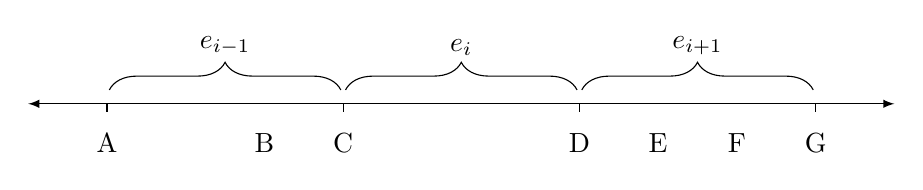
\begin{tikzpicture}
% axis
\draw[latex-latex] (0,0) -- (11,0) ;

% epoch braces
\draw [decorate,decoration={brace,amplitude=10pt} ,yshift=5pt] (1.03,0) -- (3.97,0)
  node [midway, above, yshift=9pt]{$e_{i-1}$};
\draw [decorate,decoration={brace,amplitude=10pt} ,yshift=5pt] (4.03,0) -- (6.97,0)
  node [midway, above, yshift=9pt]{$e_{i}$};
\draw [decorate,decoration={brace,amplitude=10pt} ,yshift=5pt] (7.03,0) -- (9.97,0)
  node [midway, above, yshift=9pt]{$e_{i+1}$};

% epoch boundaries
\foreach \x in  {1,4,7,10}
  \draw[shift={(\x,0)}] (0pt,0pt) -- (0pt,-3pt);

\node at (1,-0.5) {A};
\node at (3,-0.5) {B};
\node at (4,-0.5) {C};
\node at (7,-0.5) {D};
\node at (8,-0.5) {E};
\node at (9,-0.5) {F};
\node at (10,-0.5) {G};

\end{tikzpicture}

\end{document}
